\begin{flushleft}
    \huge
    \textbf{3. Design}

    \Large
    \begin{enumerate}
        \item {\Large System Flow Charts} \\
            \large
            \vspace{0.2cm}
            Below is shown the Flow Chart Overview of my Entire Project. This flowchart is very abstracted without going into
            the fine detail of each Process. \\
            
            \vspace{0.5cm}
            \centerline{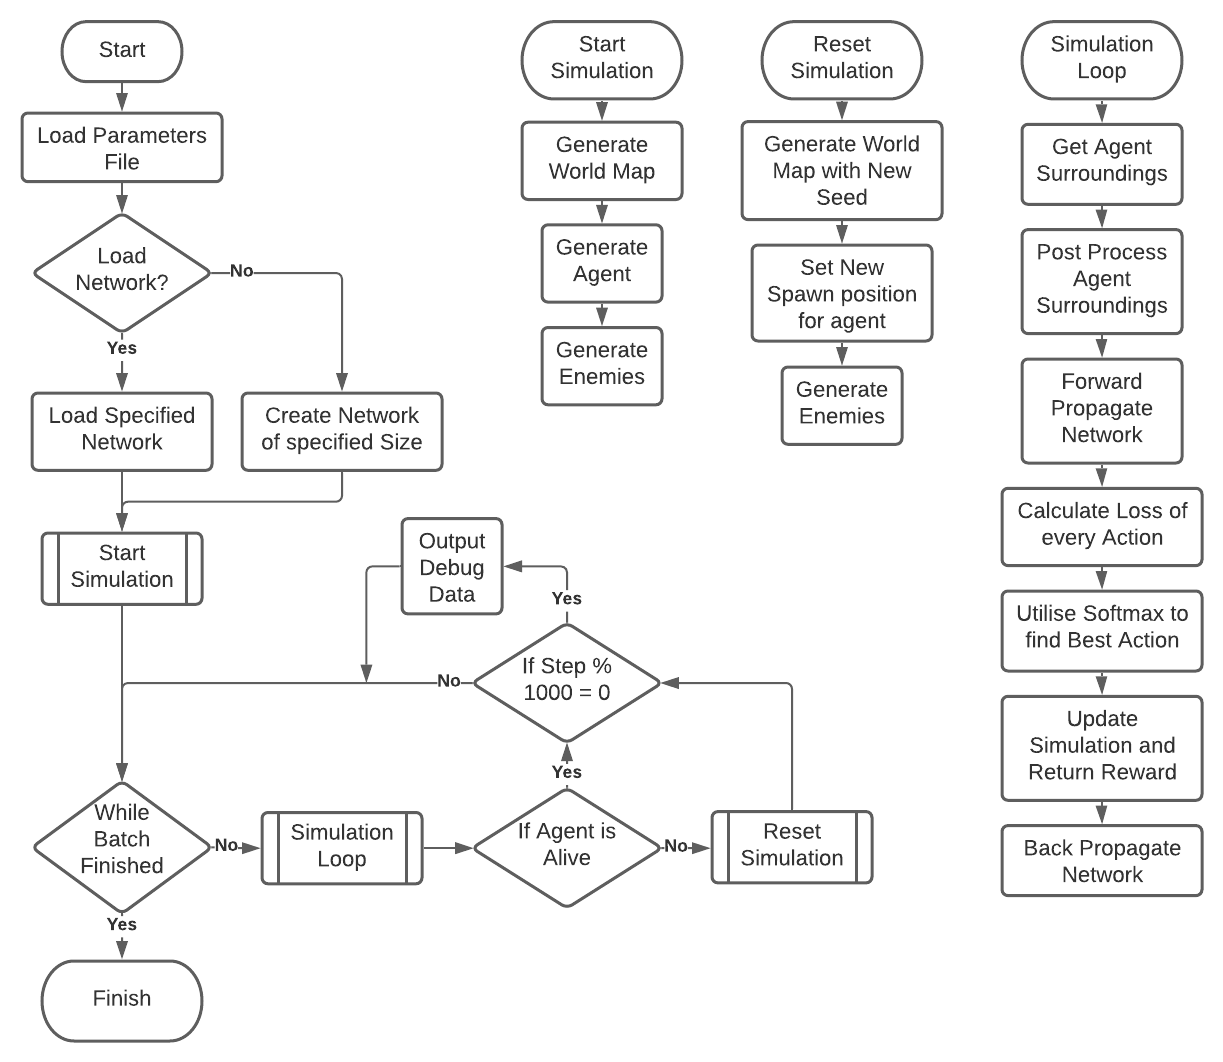
\includegraphics[width=\textwidth]{Images/Design/NEAFlowChart.png}}
            \vspace{0.5cm}

            Below is shown the Action and Reward Tree for the Agent. Any Reward is added to a Total Reward Buffer and returned
            as part of the Function. \\

            \vspace{0.5cm}
            \centerline{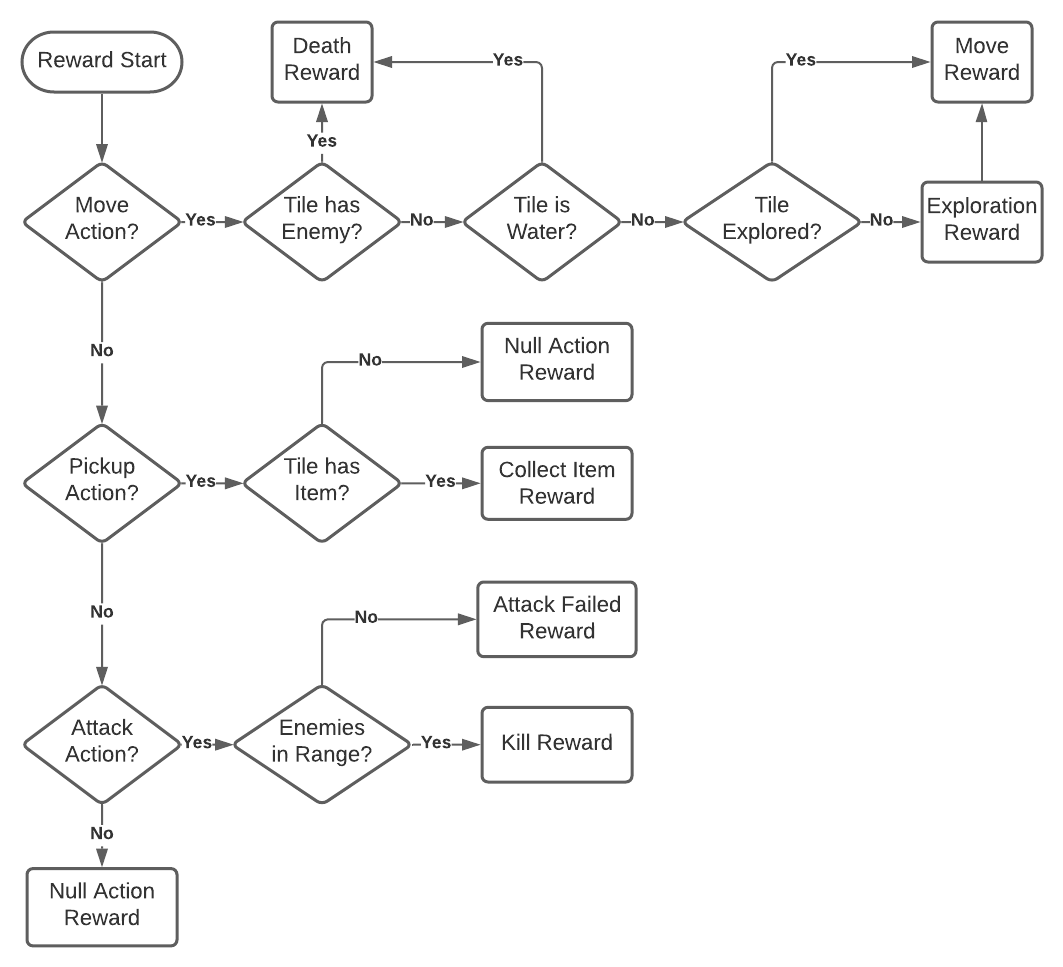
\includegraphics[width=\textwidth]{Images/Design/RewardActionStructure.png}}
            \vspace{0.5cm}

        \item {\Large Class Diagrams}
            \large
            \vspace{0.2cm}
            Below is shown the Class Diagram of the entire Technical Solution. The Data Logger is listed seperately for clarity, as
            in practice multiple sections of the Program will aggregate with it.

            \vspace{0.5cm}
            \centerline{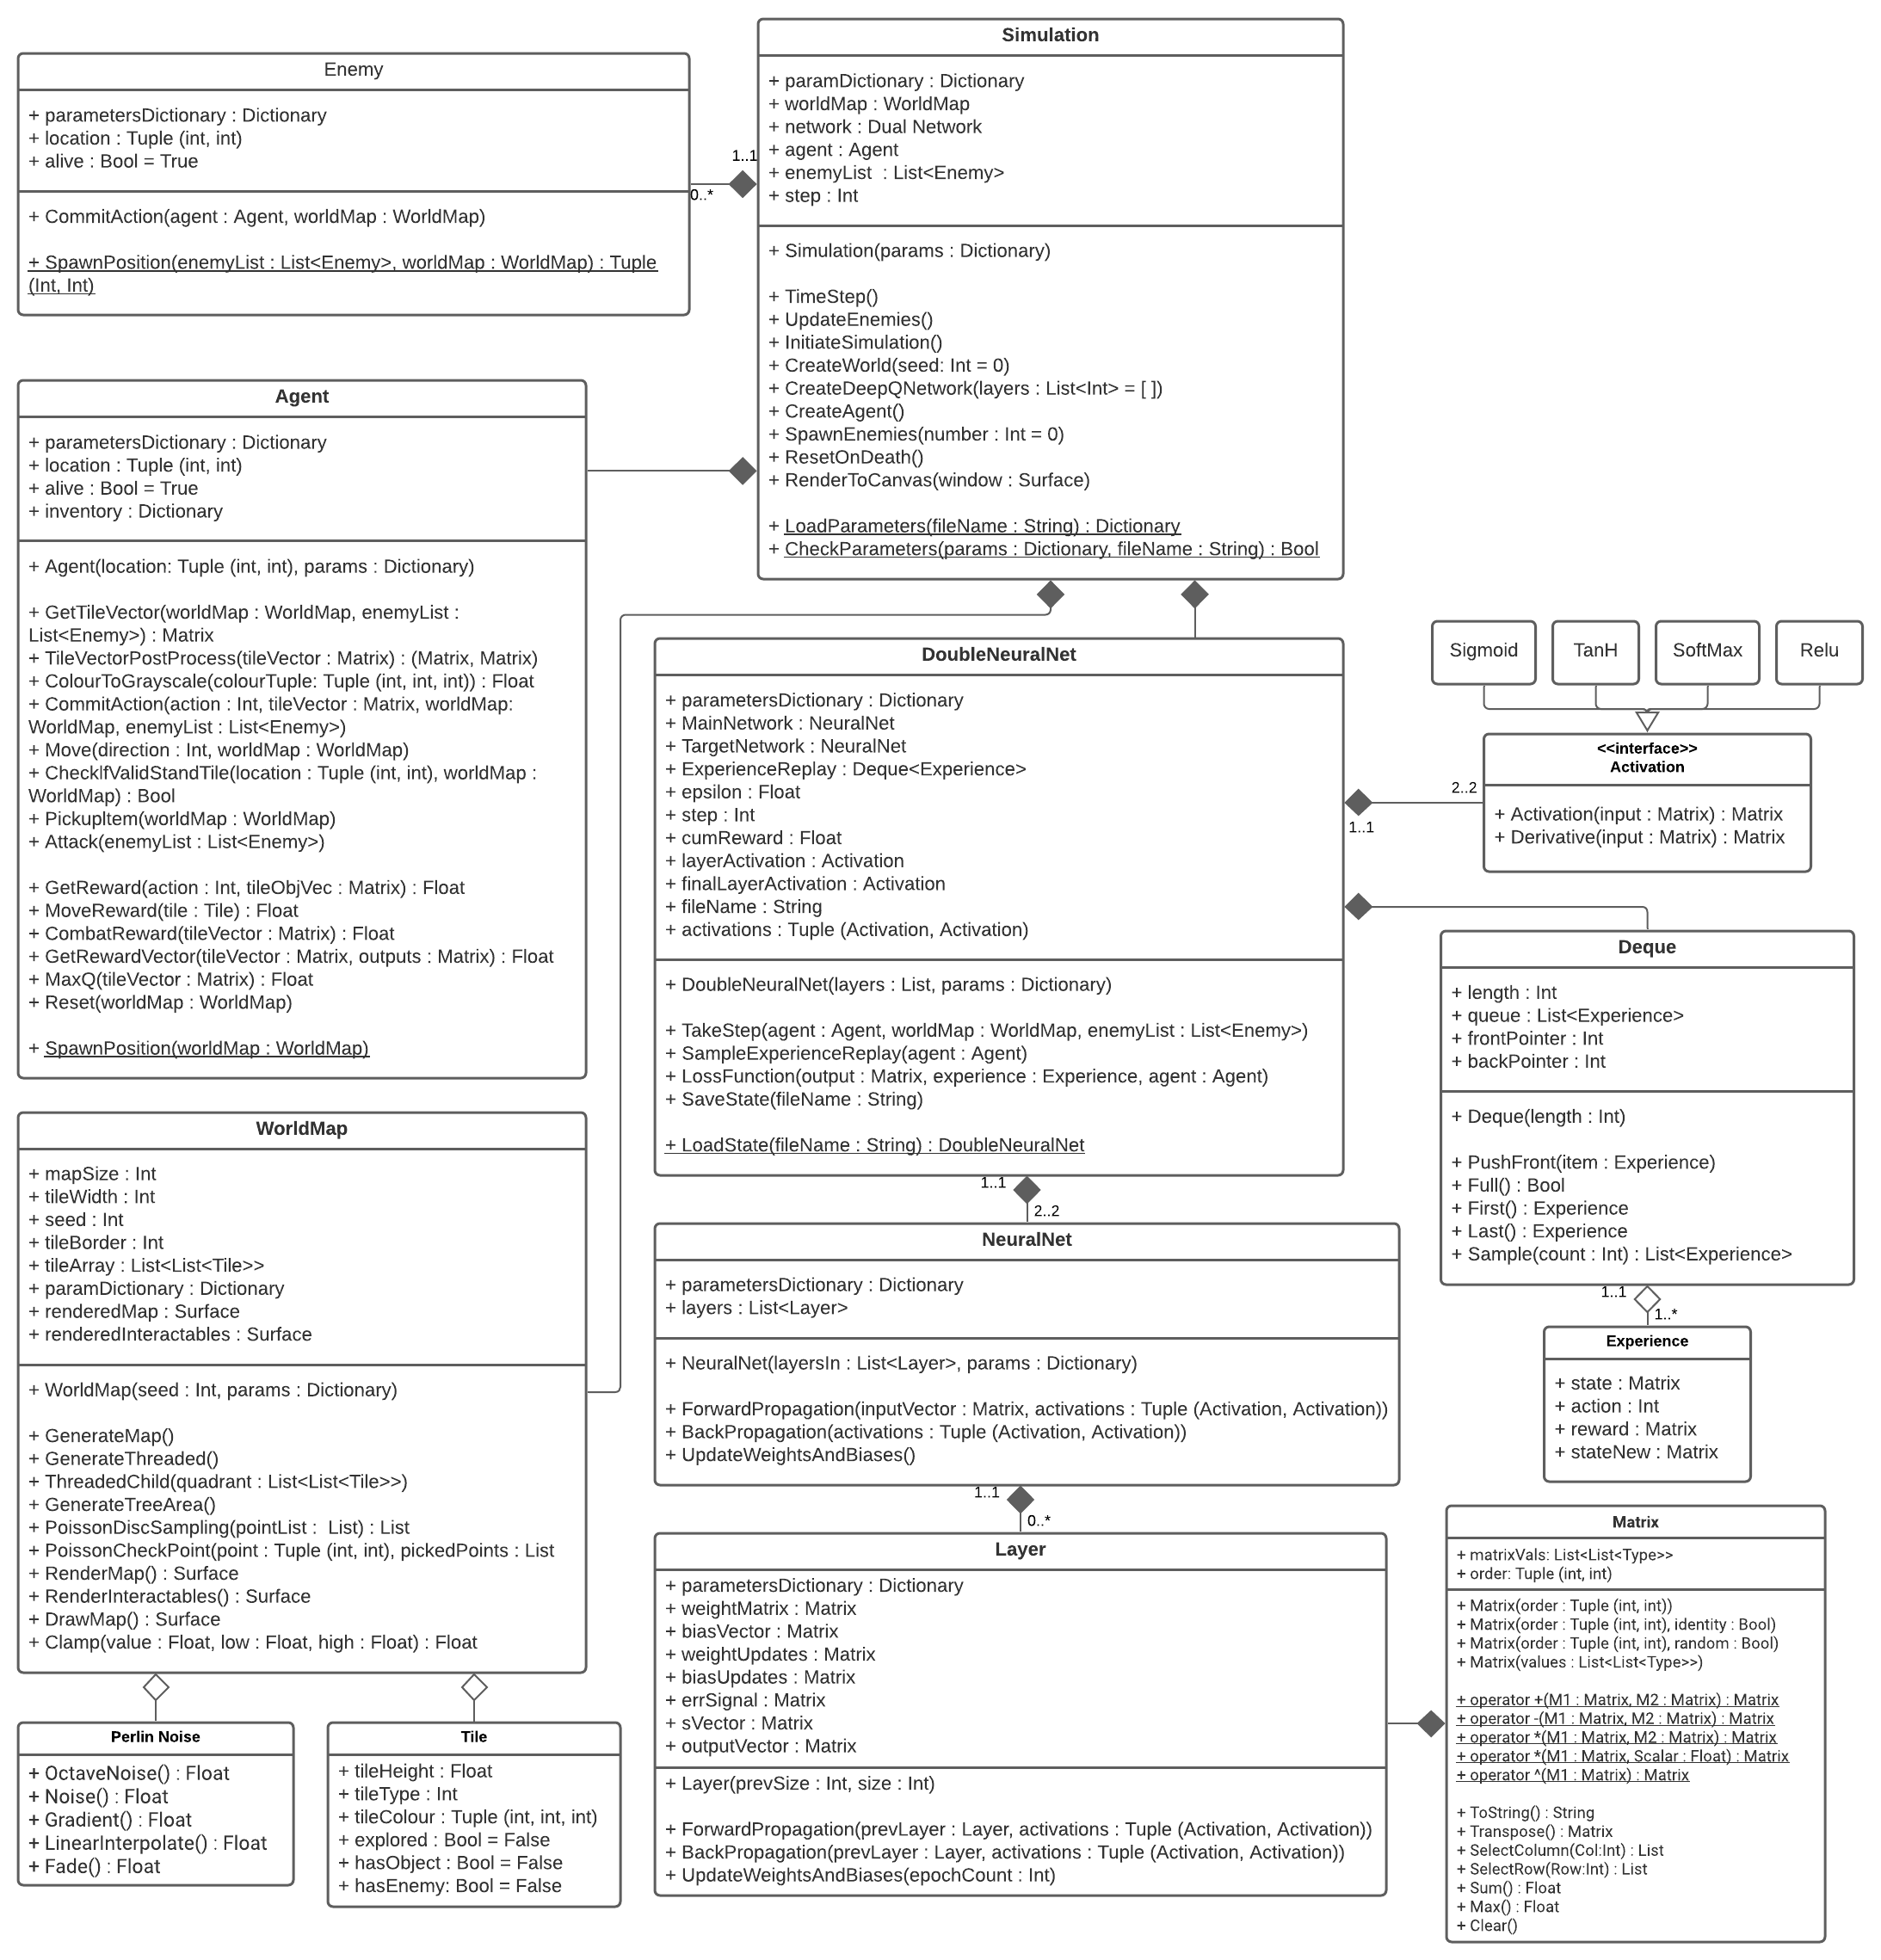
\includegraphics[width=\textwidth]{Images/Design/ClassDiagram.png}}
            \vspace{0.5cm}
            \centerline{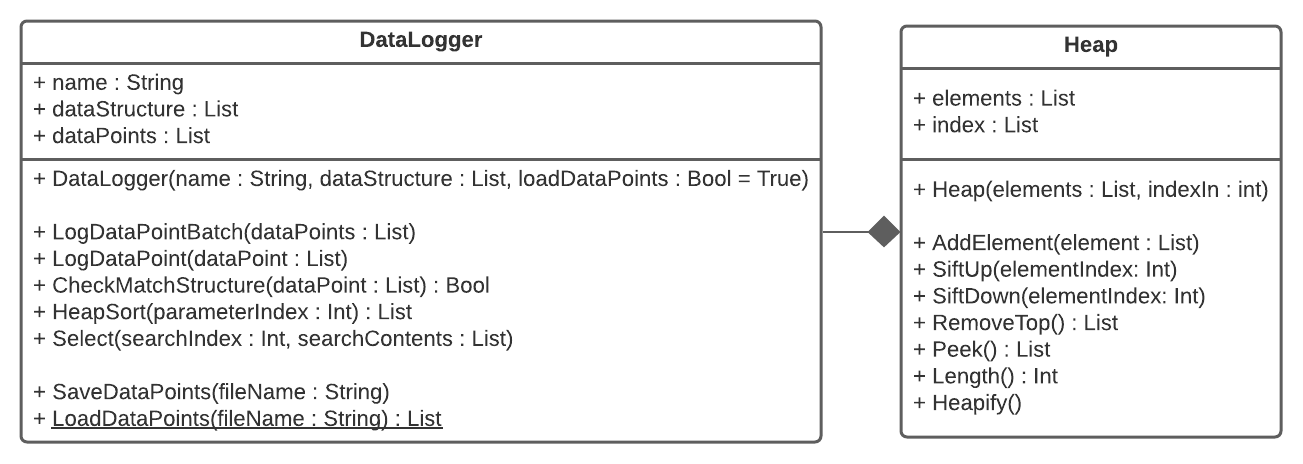
\includegraphics[width=.65\textwidth]{Images/Design/DataLoggerDiagram.png}}
            \vspace{0.5cm}

        \item {\Large Choice of Programming Language and Libraries}
            \large
            \vspace{0.2cm}  
            During my Analysis I outlined a list of possible Programming Languages and Associated Libraries. I chose Python
            and Pygame as part of my prototype. I found this combination to be very easy to use and iteratively develop my prototype.
            

        \item {\Large Description of Algorithms} \\
            \large
            \vspace{0.2cm}
            In this section, I will describe the algorithms I intend to use in my Technical Solution. I will also include generalised
            Pseudocode as part of my description.

            \begin{enumerate}[label=\arabic*)]
                \item Matrix Addition \\
                This algorithm is a Mathematical Operation to add 2 Matrices together. To Add together 2 Matrices their Orders
                must be the same. To perform the Operation you must Sum each element in Matrix A with the corresponding element 
                in Matrix B, placing the result of each Sum in the resultant Matrix.

                \vspace{0.2cm}
                \begin{pseudocode}
|\textbf{SUBROUTINE} MatrixAddition(Matrix1, Matrix2)|
    |temporaryMatrix \leftarrow \textbf{NEW} Matrix(Matrix1.Order)|
    |\textbf{FOR} Row \leftarrow 0 \textbf{TO} Matrix1.Order[0]|
        |\textbf{FOR} Column \leftarrow 0 \textbf{TO} Matrix1.Order[1]|
            |temporaryMatrix[Row, Column] \leftarrow Matrix1[Row, Column] + Matrix2[Row, Column]|
        |\textbf{END FOR}|
    |\textbf{END FOR}|
    |\textbf{RETURN} temporaryMatrix|
|\textbf{ENDSUBROUTINE}|
                \end{pseudocode}

                \vspace{0.5cm}
                \item Matrix Subtraction \\
                This algorithm is a Mathematical Operation to subtract 2 Matrices. To Subtract 2 Matrices their Orders
                must be the same. To perform the Operation you must Sum each element in Matrix A with the negative of the 
                corresponding element in Matrix B, placing the result of each Sum in the resultant Matrix.

                \vspace{0.2cm}
                \begin{pseudocode}
|\textbf{SUBROUTINE} MatrixSubtraction(Matrix1, Matrix2)|
    |temporaryMatrix \leftarrow \textbf{NEW} Matrix(Matrix1.Order)|
    |\textbf{FOR} Row \leftarrow 0 \textbf{TO} Matrix1.Order[0]|
        |\textbf{FOR} Column \leftarrow 0 \textbf{TO} Matrix1.Order[1]|
            |temporaryMatrix[Row, Column] \leftarrow Matrix1[Row, Column] - Matrix2[Row, Column]|
        |\textbf{END FOR}|
    |\textbf{END FOR}|
    |\textbf{RETURN} temporaryMatrix|
|\textbf{ENDSUBROUTINE}|
                \end{pseudocode}

                \vspace{0.5cm}
                \item Matrix Multiplication \\
                This algorithm is a Mathematical Operation to find the product of 2 Matrices. To Multiply 2 Matrices
                the number of Columns in the Matrix A must be equal to the number of Rows in Matrix B. Where Matrix A has
                dimensions of $m$ x $n$ and Matrix B has dimensions of $j$ x $k$, the resultant Matrix will have dimensions of 
                $n$ x $j$. To Multiply two Matrices, the algorithm performs the Dot Product between the Row in Matrix A and the 
                corresponding Column in Matrix B. The Dot Product is the Sum of the Products of corresponding elements.

                \vspace{0.2cm}
                \begin{pseudocode}
|\textbf{SUBROUTINE} MatrixMultiplication(Matrix1, Matrix2)|
    |tempMatrix \leftarrow \textbf{NEW} Matrix((Matrix1.Order[0], Matrix2.Order[1]))|
    |\textbf{FOR} i \leftarrow 0 \textbf{TO} Matrix1.Order[0]|
        |\textbf{FOR} j \leftarrow 0 \textbf{TO} Matrix2.Order[1]|
            |\textbf{FOR} l \leftarrow 0 \textbf{TO} Matrix.Order[1]|
                |tempMatrix[i, j] \leftarrow tempMatrix[i, j] + Matrix1[i, k] * Matrix2[k, j]|
            |\textbf{END FOR}|
        |\textbf{END FOR}|
    |\textbf{END FOR}|
    |\textbf{RETURN} tempMatrix|
|\textbf{ENDSUBROUTINE}|
                \end{pseudocode}   

                \vspace{0.5cm}
                \item Matrix Scalar Multiplication \\
                This algorithm is a Mathematical Operation to find the product between a Matrix and a Scalar.
                The result can be found by Multiplying each element of the Matrix by the Scalar Value to form the Resultant 
                Matrix.

                \vspace{0.2cm}
                \begin{pseudocode}
|\textbf{SUBROUTINE} MatrixScalarMultiplication(Scalar, Matrix)|
    |temporaryMatrix \leftarrow \textbf{NEW} Matrix(Matrix.Order)|
    |\textbf{FOR} Row \leftarrow 0 \textbf{TO} Matrix.Order[0]|
        |\textbf{FOR} Column \leftarrow 0 \textbf{TO} Matrix.Order[1]|
            |temporaryMatrix[Row, Column] \leftarrow Scalar * Matrix[Row, Column]|
        |\textbf{END FOR}|
    |\textbf{END FOR}|
    |\textbf{RETURN} temporaryMatrix|
|\textbf{ENDSUBROUTINE}|
                \end{pseudocode}   
                
                \vspace{0.5cm}
                \item Matrix Hadamard Product \\
                This algorithm is a Mathematical Operation to another way to find the product between 2 Matrices. Instead of
                applying the Dot Product between Rows and Columns, you find the product between each element in Matrix A
                with the corresponding element in Matrix B, placing the result in the resultant Matrix.

                \vspace{0.2cm}
                \begin{pseudocode}
|\textbf{SUBROUTINE} MatrixHadamardProduct(Matrix1, Matrix2)|
    |temporaryMatrix \leftarrow \textbf{NEW} Matrix(Matrix1.Order)|
    |\textbf{FOR} Row \leftarrow 0 \textbf{TO} Matrix1.Order[0]|
        |\textbf{FOR} Column \leftarrow 0 \textbf{TO} Matrix1.Order[1]|
            |temporaryMatrix[Row, Column] \leftarrow Matrix1[Row, Column] * Matrix2[Row, Column]|
        |\textbf{END FOR}|
    |\textbf{END FOR}|
    |\textbf{RETURN} temporaryMatrix|
|\textbf{ENDSUBROUTINE}|
                \end{pseudocode}   

                \vspace{0.5cm}
                \item Matrix Power \\
                This algorithm is a Mathematical Operation to find the power of a Matrix. The given Matrix needs to have square dimensions.
                The result can be found by multiplying the given Matrix by itself $n$ ammount of times where $n$ is the given power.
                
                \vspace{0.2cm}
                \begin{pseudocode}
|\textbf{SUBROUTINE} MatrixHadamardProduct(Matrix, Power)|
    |TemporaryMatrix \leftarrow \textbf{CLONE} Matrix|
    |\textbf{FOR} Row \leftarrow 0 \textbf{TO} Power - 1|
        |TemporaryMatrix \leftarrow TemporaryMatrix * Matrix|
    |\textbf{END FOR}|
    |\textbf{RETURN} TemporaryMatrix|
|\textbf{ENDSUBROUTINE}|
                \end{pseudocode}  

                \vspace{0.5cm}
                \item Matrix Transpose \\
                This algorithm is a Mathematical Operation used to Flip a Matrix across its Diagonal. The Transpose of any Matrix
                can be found by converting each Row of the Matrix into a Column. An $m$ x $n$ Matrix will turn into an $n$ x $m$ Matrix.

                \vspace{0.2cm}
                \begin{pseudocode}
|\textbf{SUBROUTINE} MatrixTranspose(Matrix)|
    |temporaryMatrix \leftarrow \textbf{NEW} Matrix(Matrix.Order)|
    |\textbf{FOR} Row \leftarrow 0 \textbf{TO} Matrix.Order[0]|
        |\textbf{FOR} Column \leftarrow 0 \textbf{TO} Matrix.Order[1]|
            |temporaryMatrix[Row, Column] \leftarrow Matrix[Column, Row]|
        |\textbf{END FOR}|
    |\textbf{END FOR}|
    |\textbf{RETURN} temporaryMatrix|
|\textbf{ENDSUBROUTINE}|
                \end{pseudocode}

                \vspace{0.5cm}
                \item Activation Function SoftMax \\
                This algorithm is a logistic function that creates a probability distribution from a set of points. This probability 
                distribution sums to 1. It applies the standard Exponential Function to each element, then normalises this value by dividing
                by the sum of all these Exponentials.

                \vspace{0.2cm}
                \begin{pseudocode}
|\textbf{SUBROUTINE} Softmax(Input)|
    |OutVector \leftarrow \textbf{NEW} Matrix(Input.Order)|
    |ExpSum \leftarrow 0|
    |\textbf{FOR} Row \leftarrow 0 \textbf{TO} Input.Order[0]|
        |ExpSum \leftarrow ExpSum + Math.exp(Input[Row, 0]|)
    |\textbf{END FOR}|
    |\textbf{FOR} Row \leftarrow 0 \textbf{TO} Input.Order[0]|
        |OutVector[Row] \leftarrow Input[Row, 0] / ExpSum|
    |\textbf{END FOR}|
    |\textbf{RETURN} OutVector|
|\textbf{ENDSUBROUTINE}|
                \end{pseudocode}

                \vspace{0.5cm}
                \item Neural Network Forward Propagation \\
                This algorithm is used to obtain the outputs of a Neural Network. It uses Matrix Multiplication to propagate the inputs
                of the network from Layer to Layer, eventually reaching the Output Layer. My Multiplying the Weight Matrix and the outputs
                of the previous Layer, and then adding the Bias. We can obtain the output of the layer.

                \vspace{0.2cm}
                \begin{pseudocode}
|\textbf{SUBROUTINE} Forward Propagation(PrevLayer, Activations, FinalLayer)|
    |WeightValueProduct \leftarrow This.WeightMatrix * PrevLayer.OutputVector|
    |This.SVector \leftarrow WeightValueProduct + This.BiasVector|
    |\textbf{IF NOT} FinalLayer|
        |This.OutputLayer \leftarrow Activations[0].Activation(SVector)|
    |\textbf{ELSE}|
        |This.OutputLayer \leftarrow Activations[1].Activation(SVector)|
    |\textbf{END IF}| 
|\textbf{ENDSUBROUTINE}|
                \end{pseudocode}

                \vspace{0.5cm}
                \item Neural Network Loss Function \\
                The algorithm for to calculate the Loss of a Dual Neural Network can calculated by using a variation of the Bellman Equation.
                The Bellman Equation is neccesary for Mathematically Optimising in this case. It determines the Value of a decision at a certain 
                point in time, in terms of the Payoff from the Inital Action and the Value of the Potential Payoff after taking that Initial
                Action. 
                
                \vspace{0.5cm}
                \item Neural Network Backwards Propagation \\
                This algorithm is used within a Neural Network to adjust its Weights and Biases, allowing it to more accurately predict the
                best outcome. In Reinforcement Learning, the Network is trained using an estimate for what is the best action given a situation.
                Using this estimate, we can train the Network to predict this outcome by converging the series of Weights and Biases towards a
                local minimum. This is done by calculating partial derivates for every weight and bias value with respect to the cost function.
                This derivative is then subtracted from the existing weight or bias, eventually converging on the best possible value.

                \vspace{0.5cm}
                \item Agent Get Tile Vector \\
                This algorithm takes the current World Data of the simulation, and produces a Vector of Tile Data surrounding the Agent. This can
                be done using a nested For Loop rather simply.

                \vspace{0.2cm}
                \begin{pseudocode}
|\textbf{SUBROUTINE} GetTileVector(WorldMap)|
    |Offset \leftarrow LoadFromParameters("DQLOffset")|
    |SideLength \leftarrow 2 * Offset + 1|
    |TileVector \leftarrow \textbf{NEW} Matrix((Math.pow(sideLength, 2), 1))|
    |Num \leftarrow 0|
    |\textbf{FOR} i \leftarrow Agent.Pos[1] - Offset \textbf{TO} Agent.Pos[1] + offset + 1|
        |\textbf{FOR} j \leftarrow Agent.Pos[0] - offset \textbf{TO} Agent.Pos[1] + offset + 1|
            |TileVector[Num, 0] \leftarrow WorldMap[j, i]|
            |Num \leftarrow Num + 1|
        |\textbf{END FOR}|
    |\textbf{END FOR}|
    |\textbf{RETURN} TileVector|
|\textbf{ENDSUBROUTINE}|
                \end{pseudocode}
                
                \vspace{0.5cm}
                \item Agent Convert to Grayscale \\
                This algorithm converts a given RGB Colour Value to the corresponding Gray Scale Value. The Red, Green and Blue elements of
                the colour value are multiplied by the specific values $0.299$, $0.587$ and $0.114$. You then sum the results, and divide by 
                $255$.

                \vspace{0.2cm}
                \begin{pseudocode}
|\textbf{SUBROUTINE} RGBToGrayscale(RGBVal)|
    |GrayscaleValue \leftarrow 0|
    |GrayscaleValue \leftarrow GrayscaleValue + (0.299 * RGBVal[0])|
    |GrayscaleValue \leftarrow GrayscaleValue + (0.587 * RGBVal[1])|
    |GrayscaleValue \leftarrow GrayscaleValue + (0.114 * RGBVal[2])|
    |\textbf{RETURN} GrayscaleValue / 255|
|\textbf{ENDSUBROUTINE}|
                \end{pseudocode}

                \vspace{0.5cm}
                \item Agent Post Process Tile Vector \\
                This algorithm will convert the Tile Vector into a Vector of Grayscale values, which can be used as the input for the Neural
                Network.

                \vspace{0.2cm}
                \begin{pseudocode}
|\textbf{SUBROUTINE} GetTileVector(TileVector)|
    |ProcessedVector \leftarrow \textbf{NEW} Matrix(TileVector.Order)|
    |\textbf{FOR} Row \leftarrow 0 \textbf{TO} TileVector.Order[0]|
        |ProcessedVector[Row, 0] \leftarrow RGBToGrayscale(TileVector[Row, 0].RGBValue)|
    |\textbf{END FOR}|
    |\textbf{RETURN} ProcessedVector|
|\textbf{ENDSUBROUTINE}|
                \end{pseudocode}
                
                \vspace{0.5cm}
                \item Agent Spawn Position \\
                This algorithm will create a list of spawnable tiles for which the Agent could spawn on, and then randomnly select a specific
                tile as its spawn position.

                \vspace{0.2cm}
                \begin{pseudocode}
|\textbf{SUBROUTINE} AgentSpawnPosition(WorldMap)|
    |SpawnList \leftarrow \textbf{NEW} List()|
    |MapSize \leftarrow LoadFromParameters("MapSize")|
    |\textbf{FOR} y \leftarrow 0 \textbf{TO} MapSize|
        |\textbf{FOR} x \leftarrow 0 \textbf{TO} MapSize|
            |\textbf{IF} WorldMap[x, y].TileType == 2|
                |SpawnList.Add([x, y])|
            |\textbf{END IF}|
        |\textbf{END FOR}|
    |\textbf{END FOR}|
    |SpawnList.Shuffle()|
    |\textbf{RETURN} SpawnList[0]|
|\textbf{ENDSUBROUTINE}|
                \end{pseudocode}

                \vspace{0.5cm}
                \item Enemy Spawn Position \\
                This algorithm will create a list of spawnable tiles for which Enemies can spawn on, then select tiles randomnly, if they dont
                already contain an enemy or the agent it will create an Enemy Object with that position. It will do this $n$ ammount of times 
                where $n$ is the limit to how many enemies can spawn.
                
                \vspace{0.2cm}
                \begin{pseudocode}
|\textbf{SUBROUTINE} EnemySpawnPosition(WorldMap, EnemyList)|
    |SpawnList \leftarrow \textbf{NEW} List()|
    |EnemyLocationList \leftarrow \textbf{NEW} List()|
    |MapSize \leftarrow LoadFromParameters("MapSize")|
    |\textbf{FOR} y \leftarrow 0 \textbf{TO} MapSize|
        |\textbf{FOR} x \leftarrow 0 \textbf{TO} MapSize|
            |\textbf{IF} WorldMap[x, y].TileType == 2|
                |SpawnList.Add([x, y])|
            |\textbf{END IF}|
        |\textbf{END FOR}|
    |\textbf{END FOR}|
    |SpawnList.Shuffle()|
    |\textbf{IF} SpawnList[0] \textbf{IN} EnemyLocationList|
        |\textbf{RETURN NONE}|
    |\textbf{ELSE}|
        |\textbf{RETURN} SpawnList[0]|
    |\textbf{END IF}|
    |\textbf{RETURN} SpawnList[0]|
|\textbf{ENDSUBROUTINE}|
                \end{pseudocode}

                \vspace{0.5cm}
                \item Enemy Move \\
                The algorithm I have designed for the Enemy Pathfinding is rather simple, and wont take up much runtime in my solution.
                First it calculates the distance between itself and the Agent in both Axis. The Enemy will then converge upon the Agents
                position by moving in the direction with the greatest distance, effectively finding the nearest diagonal and following it.

                \vspace{0.2cm}
                \begin{pseudocode}
|\textbf{SUBROUTINE} EnemyMove(Agent, WorldMap)|
    |XDifference \leftarrow Agent.Pos[0] - This.Pos[0]|
    |YDifference \leftarrow Agent.Pos[1] - This.Pos[0]|

    |\textbf{IF} XDifference == 0 \textbf{AND} YDifference == 0|
        |Agent.Alive = False|
        |\textbf{RETURN}|
    |\textbf{END IF}|

    |\textbf{IF} abs(XDifference) > abs(YDifference)|
        |\textbf{IF} XDifference > 0|
            |This.Pos[0] \leftarrow This.Pos[0] + 1|
        |\textbf{ELSE}|
            |This.Pos[0] \leftarrow This.Pos[0] - 1|
        |\textbf{END IF}|
    |\textbf{ELSE IF} abs(XDifference) < abs(YDifference)|
        |\textbf{IF} YDifference > 0|
            |This.Pos[1] \leftarrow This.Pos[1] + 1|
        |\textbf{ELSE}|
            |This.Pos[1] \leftarrow This.Pos[1] - 1|
        |\textbf{END IF}|
    |\textbf{END IF}|
|\textbf{ENDSUBROUTINE}|
                \end{pseudocode}
                
                \vspace{0.5cm}
                \item Poisson Disc Sampling \\
                Poisson Disc Sampling is used to sample a set of points in N Dimensional Space. It takes two parameters, $r$ and $k$, where
                $r$ is the minimum distance a specified point must be from every other point, and $k$ is the limit of samples to choose
                before rejection. It starts by creating an N Dimensional Grid which accelerates spacial searches. An initial sample is then
                chosen and inserted into the grid. It then chooses a random point, and determines if it is greater than $r$ range from every 
                other point in the grid. This can easily be acomplished using the previously defined Grid. If after $k$ attempts, no point is
                found then the search is concluded.

                \vspace{0.2cm}
                \begin{pseudocode}
|\textbf{SUBROUTINE} PoissonDiscSampling(PointList)|
    |KVal \leftarrow LoadFromParameters("PoissonKVal")|
    |MapSize \leftarrow LoadFromParameters("MapSize")|
    |PickedPoints \leftarrow \textbf{NEW} Grid(MapSize, MapSize)|
    |SampleNum \leftarrow LoadFromParameters("MapSize")|
    |\textbf{WHILE} SampleNum <= KVal|
        |Sample \leftarrow PointList[RandomInt(0, PointList.Length - 1)]|
        |Result \leftarrow CheckPointDistance(Sample, PickedPoints)|
        |\textbf{IF} Result == True|
            |PickedPoints[Sample[0], Sample[1]] \leftarrow = True|
            |SampleNum \leftarrow 0|
            |\textbf{CONTINUE}|
        |\textbf{ELSE}|
            |SampleNum \leftarrow SampleNum + 1|
            |\textbf{CONTINUE}|
        |\textbf{END IF}|
    |\textbf{END WHILE}|
    |\textbf{RETURN} PickedPoints|
|\textbf{ENDSUBROUTINE}|
                \end{pseudocode}
                
                \vspace{0.5cm}
                \item Perlin Noise \\
                Perlin Noise is a method of generating a procedural texture depending upon input parameters. It defines an n-dimensional
                grid of Vectors, each grid intersection contains a fixed, random unit vector. To sample Perlin Noise, the grid cell which
                the point lies in must be found. The Vectors between the sampled point, and the corners of the cell. We then take the Dot
                Product between these new Vectors, and the Vectors applied to the intersections. In 2d Space this leaves us with 4 Values.
                We then use an Interpolation function to Interpolate between the 4 Values. 
            
                \vspace{0.2cm}
                \begin{pseudocode}
|PermTable \leftarrow [1 \rightarrow 255].Shuffle() * 2|

|\textbf{SUBROUTINE} PerlinNoise(X, Y)|
    |XFloor \leftarrow Math.floor(X)|
    |YFloor \leftarrow Math.floor(Y)|

    |G1 \leftarrow PermTable[PermTable[XFloor] + YFloor]|
    |G2 \leftarrow PermTable[PermTable[XFloor + 1] + YFloor]|
    |G3 \leftarrow PermTable[PermTable[XFloor] + YFloor + 1]|
    |G4 \leftarrow PermTable[PermTable[XFloor + 1] + YFloor + 1]|

    |XExact \leftarrow X - XFloor|
    |YExact \leftarrow Y - YFloor|

    |D1 \leftarrow Grad(G1, XFloor, YFloor)|
    |D2 \leftarrow Grad(G2, XFloor - 1, YFloor)|
    |D3 \leftarrow Grad(G3, XFloor, YFloor - 1)|
    |D4 \leftarrow Grad(G4, XFloor - 1, YFloor - 1)|

    |U \leftarrow Fade(XFloor)|
    |V \leftarrow Fade(YFloor)|

    |XInterpolated \leftarrow Lerp(U, D1, D2)|
    |YInterpolated \leftarrow Lerp(U, D3, D4)|

    |\textbf{RETURN} Lerp(V, XInterpolated, YInterpolated)|
|\textbf{ENDSUBROUTINE}|

|\textbf{SUBROUTINE} Grad(Hash, X, Y)|
    |Temp \leftarrow Hash BITWISEAND 3|
    |\textbf{IF} Temp == 0|
        |\textbf{RETURN} X + Y|
    |\textbf{ELSE IF} Temp == 1|
        |\textbf{RETURN} -X + Y|
    |\textbf{ELSE IF} Temp == 2|
        |\textbf{RETURN} X - Y|
    |\textbf{ELSE IF} Temp == 3|
        |\textbf{RETURN} -X - Y|
    |\textbf{ELSE}|
        |\textbf{RETURN} 0|
    |\textbf{END IF}|
|\textbf{ENDSUBROUTINE}|

|\textbf{SUBROUTINE} Lerp(Ammount, Left, Right)|
    |\textbf{RETURN} ((1 - Ammount) * Left + Ammount * Right)|
|\textbf{ENDSUBROUTINE}|

|\textbf{SUBROUTINE} Fade(T)|
    |\textbf{RETURN} T * T * T * (T * (T * 6 - 15) + 10)|
|\textbf{ENDSUBROUTINE}|
                \end{pseudocode}

                \vspace{0.5cm}
                \item Octave Perlin Noise \\
                Octave Perlin Noise takes the existing Perlin Noise algorithm, but adds rescaled clones of itself into itself, to create
                what is known as Fractal Noise. Creating this Fractal Noise is common practice because it reduces the sharp edges encountered
                with just the regular Perlin Noise Algorithm.

                \vspace{0.2cm}
                \begin{pseudocode}
|\textbf{SUBROUTINE} OctaveNoise(X, Y, Octaves, Persistence)|
    |Total \leftarrow 0|
    |Frequency \leftarrow 1|
    |Amplitude \leftarrow 1|
    |MaxValue \leftarrow 0|

    |\textbf{FOR} i \leftarrow 0 \textbf{TO} Octaves|
        |Total \leftarrow Total + (PerlinNoise(X * Frequency, Y * Frequency) * Amplitude|

        |MaxValue \leftarrow MaxValue + Amplitude|

        |Amplitude \leftarrow Amplitude * Persistence|
        |Frequency \leftarrow Frequency * 2|
    |\textbf{END FOR}|

    |\textbf{RETURN} Total / MaxValue|
|\textbf{ENDSUBROUTINE}|            
                \end{pseudocode}

                \item Heap Heapify \\
                The Heapify algorithm converts a Binary Tree of values into a valid Heap. The Heap Property is defined in Description of Data
                Structures below. This algorithm works by repeatedly performing Sift Down Operations for \textbf{$\lfloor$(N-1)/2$\rfloor$} times.
                Where N is the Number of elements in the Tree. A Sift Down Operation will swap elements which don't conform to the Heap Property.
                This operation relys on the fact that Children of an Index are located at \textbf{2i + 1} and \textbf{2i + 2}.
                \vspace{0.2cm}

                \begin{pseudocode} 
|\textbf{SUBROUTINE} Heapify()|
    |\textbf{FOR} i \leftarrow $\lfloor$(HeapList.Length-1)/2$\rfloor$ \textbf{TO} 0 \textbf{STEP} -1|
        |SiftDown(i)|
    |\textbf{END FOR}|
|\textbf{ENDSUBROUTINE}| 

|\textbf{SUBROUTINE} SiftDown(RootIndex)|
    |IsHeap \leftarrow \textbf{FALSE}|
    |End \leftarrow HeapList.Length - 1|

    |\textbf{WHILE} (2 * RootIndex) + 1 <= End|
        |ChildIndex = (RootIndex * 2) + 1|
        |\textbf{IF} ChildIndex <= End \textbf{AND} HeapList[ChildIndex] < HeapList[ChildIndex + 1]|
            |ChildIndex \leftarrow ChildIndex + 1|
        |\textbf{END IF}|
        |\textbf{IF} HeapList[RootIndex] < HeapList[ChildIndex]|
            |TempSwap \leftarrow HeapList[ChildIndex]|
            |HeapList[ChildIndex] \leftarrow HeapList[RootIndex]|
            |HeapList[RootIndex] \leftarrow TempSwap|
        |\textbf{ELSE}|   
            |\textbf{BREAK}|
        |\textbf{END IF}|
|\textbf{ENDSUBROUTINE}| 
                \end{pseudocode}

                \vspace{0.5cm}
                \item Heap Extraction \\
                This algorithm extracts the Root Element from a valid Heap. It does this by swapping the Root Element and Final Element, and then
                popping the new Final Element (Originally the Root) from the list. 
                \vspace{0.2cm}

                \begin{pseudocode}
|\textbf{SUBROUTINE} RemoveTop()|
    |TempSwap \leftarrow HeapList[-1]|
    |HeapList[-1] \leftarrow HeapList[0]|
    |HeapList[0] \leftarrow TempSwap|
    |ReturnItem \leftarrow HeapList.Pop()|

    |Heapify()|

    |\textbf{RETURN} ReturnItem|
|\textbf{ENDSUBROUTINE}| 
                \end{pseudocode}

                \vspace{0.5cm}
                \item Heap Sort \\
                The Heap Sort algorithm relys on the prior two algorithms to fully order a list in Worst and Best case $O(nlog(n))$ Time Complexity. It 
                is also $O(1)$ Space Complexity due to it being an In-Place Sorting algorithm. The sort will iteratively shrink the unsorted region by 
                performing the following steps: Apply Heapify to the Unsorted Region, Extract the Root Element from the Heap, Insert the Extracted Element 
                at the end of the Unsorted Region. This allows it to be In-Place because it never requires extra space.
                \vspace{0.2cm}

                \begin{pseudocode}
|\textbf{SUBROUTINE} HeapSort()|
    |SortedList \leftarrow \textbf{NEW} List()|
    |Heap \leftarrow \textbf{NEW} Heap(DataPoints)|

    |\textbf{WHILE} Heap.Size() - 1 >= 0|
        |SortedList.Append(Heap.RemoveTop)|
    |\textbf{END FOR}|

    |\textbf{RETURN} SortedList|
|\textbf{ENDSUBROUTINE}|
                \end{pseudocode}

                \vspace{0.5cm}
            \end{enumerate}

        \vspace{0.5cm}
        \item {\Large Description of Data Structures} \\
            \large
            \vspace{0.2cm}
            \begin{enumerate}
                \item {\Large Matrices} \\
                As part of developing a Neural Network, I will extensively use Matrices, as they are an integral part of the algorithms
                used for Machine Learning. After creating a prototype Matrix class as part of my prototype, I will represent it in the
                same format. A Matrix can be represented simply using a 2D Array, but they can have Mathematical Operations performed
                between them. Explanations and the formulae can be found in the Modelling of the Problem Analysis Section. \\
                \vspace{0.2cm}
                To avoid repeating code in some places, Matrices will have multiple Constructors. The main Constructors are in the form 
                of an (Int, Int) Tuple, or an pre-existing 2D Array. Other less used examples could be an Integer for creating 
                a Vector of that length. \\
                \vspace{0.2cm}
                Operator Overloading will be useful when implementing a Matrix Class, as it allows classes to have implementations for
                operators such as Multiplication, Addition, Subtraction etc. This avoids the need to rely on Static Methods for Operator
                Implementations and makes code much more readable overall. \\
                \vspace{0.2cm}
                As part of a Neural Network Matrices are used heavily in the calculations. So it will be important to optimise the
                implemented algorithms to make sure their Algorithmic Time Complexity is minimised. \\

                \vspace{0.5cm}
                \item {\Large Double Ended Queue} \\
                A Double Ended Queue (Commonly referred to as a {\textbf{Deque}}) is an Abstract Data Type, which is a generalisation of 
                a Queue. Elements can be added to the Front/Head or Back/Tail. Deques are commonly implemented using an Array, and two
                pointers, one for Front and Back.

                \vspace{0.5cm}
                \item {\Large Tile} \\
                A Tile is used to store specific location Data as part of the World Map. It can be initialised without values, and is
                then populated with the relevant information. Methods are attatched to this Class to Add/Remove Items and Enemies as needed.
                Allowing for the Agent when getting Tile data to get relevant and accurate information.

                \vspace{0.5cm}
                \item {\Large Experience} \\
                An Experience is used to store data for Experience Replay. It is an Empty Class with no Methods. This includes the State, 
                Action, NewState and Reward, all at the time of assignment. This is used in conjunction with the Experience Replay 
                Algorithm, described above.

                \vspace{0.5cm}
                \item {\Large Heap} \\
                A Heap is specialised Binary Tree which satisfies the \textbf{Heap Property}: such that for all nodes with Parents, the
                Parent has a greater value than the Child. A Heap is used as part of a Heap Sort, an $O(nlog(n))$ Sorting Algorithm. The
                highest priority element is always stored at the Root, with the tree of the structure being considered "Partialy Ordered".
                Heaps can be stored in an Array, with the Root element at Index 0. Children of an Index are located at \textbf{2i + 1} and
                \textbf{2i + 2}. The Parent of an Index is located at \textbf{$\lfloor$(i-1)/2$\rfloor$}.
            \end{enumerate}

        \vspace{0.5cm}
        \item {\Large File Structure} \\
            \large
            \vspace{0.2cm}
            \begin{enumerate}
                \item {\Large User Defined Parameters} \\
                As part of my Technical Solution, the User will be able to modify the parameters which dynamically modifies the Simulation
                and the Structure of the Double Neural Network. The file is stored in a Json format (Java Script Object Notation).
                This allows the File to be Human Readable, and easily editable. Each parameter will also have a defined Range alongside it.
                The program will throw an error if the parameter is outside the specified range. Below is a table of the Parameters used in
                the Technical Solution, alongside their respective Ranges. \\

                \vspace{0.5cm}

                \normalsize
                \begin{longtable}{| C{4cm} | C{2cm} | C{1.5cm} | C{8cm} |}
                    \hline
                    Name in Json & Data Type & Range & Description \\
                    \hline\hline
                    EnterValues & Int & 0 - 1 & The program will ask you to enter values if this is 1 \\
                    \hline
                    GenerateThreaded & Int & 0 - 1 & The program will generate the Terrain using Multiple Threads \\
                    \hline
                    EnableEnemies & Int & 0 - 1 & Toggled Enable Enemies Option. \\
                    \hline
                    SaveWeights & Int & 0 - 1 & Toggled Save Network Weights Option. \\
                    \hline
                    StepDelay & Float & 0 - \infty & The time delay each step. \\
                    \hline
                    Debug & Int & 0 - 1 & Toggled Debug Option. \\
                    \hline
                    DebugScale & Int & 1 - 4 & The scale of the Debug side extension. \\
                    \hline
                    WorldSize & Int & 16 - 1024 & The size the of the World in Tiles. Must be a Multiple of 2. \\
                    \hline
                    TileWidth & Int & 1 - 8 & The Width and Height of each Tile. \\
                    \hline
                    TileBorder & Int & 0 - 3 & The Pixel Border surrounding Tiles. \\
                    \hline
                    OctavesTerrain & Int & 1 - 20 & The Perlin Noise Octave Value for World Generation. \\
                    \hline
                    PersistenceTerrain & Float & 0 - 1 & The Perlin Noise Persistence Value for World Generation. \\
                    \hline
                    WorldScale & Float & 0.1 - 10 & The Perlin Noise Scale Value for World Generation. \\
                    \hline
                    OctavesTrees & Int & 1 - 20 & The Perlin Noise Octave Value for Trees \\
                    \hline
                    PersistenceTrees & Float & 0 - 1 & The Perlin Noise Persistence Value for generating the Trees. \\
                    \hline
                    PoissonKVal & Int & 0 - \infty & The K Value for Poisson Disc Sampling. \\
                    \hline
                    TreeSeedOffset & Int & 0 - \infty & The Seed offset for generating the Trees. \\
                    \hline
                    TreeHeight & Float & 0 - 1 & The difference between Min Tree spawning height and Max Tree spawning height. \\
                    \hline
                    InteractableTileBorder & Int & 0 - 3 & The Pixel Border surrounding Interactables. \\
                    \hline
                    TreeBeachOffset & Float & 0 - 1 & The height difference from Beaches which Trees will Spawn. \\
                    \hline
                    Grayscale & Int & 0 - 1 & Toggled Grayscale Terrain Option. \\
                    \hline
                    Water & Float & 0 - 1 & The cuttoff values for Water. \\
                    \hline
                    Coast & Float & 0 - 1 & The cuttoff values for Coast. \\
                    \hline
                    Grass & Float & 0 - 1 & The cuttoff values for Grass. \\
                    \hline
                    Mountain & Float & 0 - 1 & The cuttoff values for Mountains. \\
                    \hline
                    TreeType & String & 0 - 1 & The internally used Inventory name for collected Trees. \\
                    \hline
                    StartEnemyCount & Int & 0 - \infty & The maximum count of Enemies to Spawn upon the creation of a new Map. \\
                    \hline
                    ColourWater & [Int, Int, Int] & 0 - 255 & The display Colour of Water. \\
                    \hline
                    ColourCoast & [Int, Int, Int] & 0 - 255 & The display Colour of Coast. \\
                    \hline
                    ColourGrass & [Int, Int, Int] & 0 - 255 & The display Colour of Grass. \\
                    \hline
                    ColourMountain & [Int, Int, Int] & 0 - 255 & The display Colour of Mountains. \\
                    \hline
                    ColourTree & [Int, Int, Int] & 0 - 255 & The display Colour of Trees. \\
                    \hline
                    ColourPlayer & [Int, Int, Int] & 0 - 255 & The display Colour of the Agent. \\
                    \hline
                    ColourEnemy & [Int, Int, Int] & 0 - 255 & The display Colour of Enemies. \\
                    \hline
                    MoveReward & Float & -1 - 1 & The Reward Gained when the Agent Moves. \\
                    \hline
                    CollectItemReward & Float & -1 - 1 & The Reward Gained when the Agent collects an Item. \\
                    \hline
                    DeathReward & Float & -1 - 1 & The Reward Gained when the Agent Dies through any means. \\
                    \hline
                    ExploreReward & Float & -1 - 1 & The Reward Gained when the Agent moves into a Tile which hasnt been Visited yet. \\
                    \hline
                    AttackReward & Float & -1 - 1 & The Reward Gained when the Agent successfully Attacks an Enemy. \\
                    \hline
                    AttackFailedReward & Float & -1 - 1 & The Reward Gained when the Null Action is chosen. \\
                    \hline
                    NoopReward & Float & -1 - 1 & The Reward Gained when the Null Action is chosen. \\
                    \hline
                    TargetReplaceRate & Int & 5 - 300 & Replace Rate for Target Neural Network. \\
                    \hline
                    EREnabled & Int & 0 - 1 & Wether Experience Replay is Enabled or Disabled. \\
                    \hline
                    ERBuffer & Int & 1k - 10k & The size of the Experience Replay Buffer. \\
                    \hline
                    ERSampleRate & Int & 1 - 100 & The ammount of steps between each Experience Replay sample. \\
                    \hline
                    ERSampleSize & Int & 10 - 1000 & The ammount of samples taken from the Experience Replay Buffer. \\
                    \hline
                    DeepQLearningLayers & [Int, ..., Int] & 0 - 256 & List of Integers defining the size of each Layer in the Neural Network. \\
                    \hline
                    DQLEpoch & Int & 10 - 1000 & The ammount of steps per Weight and Bias Update, along with Network Saving and Debug Output \\
                    \hline
                    DQLearningMaxSteps & Int & 1000 - \infty & Maximum steps the Simulation will run for. \\
                    \hline
                    DQLOffset & Int & 1 - 10 & The square radius around the agent which is sampled for the Input vector, must be the root of the 
                    Input Layers size. \\
                    \hline
                    DQLEpsilon & Float & 0 - 1 & The initial Probability that the Agent will favour a Random Action over the predicted Action \\
                    \hline
                    DQLEpsilonRegression & Float & 0 - 1 & The rate at which Epsilon will decrease, Epsilon is multiplied every step by this number \\
                    \hline
                    DQLLearningRate & Float & 0 - 1 & The Learning Rate of the Neural Network. Higher values will cause more drastic changes during
                    Back Propagation. \\
                    \hline
                    DQLGamma & Float & 0 - 1 & The Discount for future gained Reward \\
                    \hline
                \end{longtable}

                \vspace{0.5cm}
                \item {\Large .dqn Files} \\
                \vspace{0.2cm}
                DQN Files are used to store all Data relating to the Dual Neural Network. It is a Binary File. It contains all Layer Data, along
                with Experience Replay Data, the activations being used, and other important data.

                \vspace{0.5cm}
                \item {\Large .data Files} \\
                \vspace{0.2cm}
                Data Files are used to store all data points created by the Data Loggers. They are Binary Files and are individually created per Data
                Logger.
            
                \vspace{0.5cm}
            \end{enumerate}
        

    \end{enumerate}
    \vspace{0.1cm}
\end{flushleft}